\documentclass[a4paper,11pt,utf8]{article}

\usepackage[utf8]{inputenc}
\usepackage[T1]{fontenc}
\usepackage{amsmath, amssymb, amsthm}
\usepackage{mathtools}
\usepackage{graphicx}
\usepackage{hyperref}
\usepackage{CJKutf8}
\usepackage{ctex}
\usepackage{geometry}
\usepackage{fancyhdr}
\usepackage{titling}
\usepackage{enumitem}
\usepackage{mdframed}
\usepackage{tcolorbox}
\usepackage{tikz}
\usepackage{forest}
\usepackage{multicol}

\usetikzlibrary{arrows.meta, positioning, shapes.geometric, calc, quotes, trees}

\renewcommand{\contentsname}{\text{Contents 目录}}
\renewcommand{\headrulewidth}{0.4pt}
\renewcommand{\footrulewidth}{0.4pt}

\newcommand{\newindent}{\\ \hspace*{\parindent}}
\newcommand{\lineindent}{\hspace*{\parindent}}


\geometry{
    left=1cm,
    right=1cm,
    top=1.5cm,
    bottom=1.5cm,
    includehead,
    includefoot
}

\title{\text{Graph Algorithms Summary}}
\author{玄风}
\newcommand{\copyrighttext}{\text{©玄风 2025 ALL RIGHTS RESERVED.}}
\date{}

\setlength{\headheight}{13.6pt}
\pagestyle{fancy}
\fancyhf{}
\fancyhead[R]{\thepage}
\fancyhead[L]{\nouppercase{\leftmark}}
\fancyfoot[L]{\text{Graph Algorithms}}
\fancyfoot[R]{\text{Updated: \today}}


\pretitle{\begin{center}\Huge\bfseries}
    \posttitle{\par\end{center}}
    \preauthor{\vfill\begin{center}\large}
    \postauthor{
      \\[1em]
      \normalfont\scriptsize \copyrighttext
      \end{center}
    }

\begin{document}

\maketitle
\thispagestyle{empty}
\newpage
\pagenumbering{roman}
\tableofcontents
\thispagestyle{empty}
\newpage

\clearpage
\pagenumbering{arabic}
\setcounter{page}{1} 

% start here
\section{Basic Knowledge 基础知识}
\begin{multicols}{2}
  A graph $G = (V,E)$ consists of a: node quantity $V$ and edge quantity $E$. \newindent
  Undirected graph: $E \subseteq \{\{u,v\} \mid u,v \in V\}$. \newindent
  Directed graph: $E \subseteq V \times V = \{(u,v) \mid u,v \in V\}$. \newindent
  \columnbreak
  Knote = node, Kante = edge. \newindent
  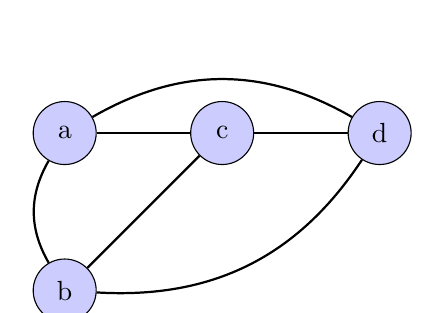
\begin{tikzpicture}[node distance=2cm,every node/.style={circle,draw,minimum size=8mm,fill=blue!20},edge/.style={thick,black}]
    \node (a) {a};
    \node (b) [below of=a] {b};
    \node (c) [right of=a] {c};
    \node (d) [right of=c] {d};

    \draw[edge] (a) to[bend right=30] (b);
    \draw[edge] (a) -- (c);
    \draw[edge] (b) -- (c);
    \draw[edge] (b) to[bend right=30] (d);
    \draw[edge] (c) -- (d);
    \draw[edge] (a) to[bend left=30] (d);
  \end{tikzpicture} \\
  \lineindent $V=\{a,b,c,d\}$ \\
  \lineindent $E=\{\{a,b\},\{a,c\},\{a,d\},\{b,c\},\{b,d\},\{c,d\}\}$
\end{multicols}
% end here


\end{document}
